\documentclass[12pt,a4paper,portrait]{beamer}
\usetheme{default}
\usecolortheme{crane}
\usepackage{polski}
\usepackage[utf8]{inputenc}
\inputencoding{utf8}
\usepackage[polish]{babel}
\usepackage{amsmath}
\usepackage{amsfonts}
\usepackage{amssymb}
\usepackage{graphicx}
\usepackage{ragged2e}
\usepackage{multimedia}
%\usepackage{movie15}
%\usepackage{hyperref}
\usepackage{listings}

\author[AW]{Adam Wolniakowski}
\institute[WM PB]{Politechnika Białostocka}
\title[PhD]{Automatyczne projektowanie chwytaków robotów w kontekście zadań}
\date{22 października, 2014}
%\logo{\includegraphics[width=1cm]{logo.png}}

\begin{document}

\section{Start}
\begin{frame}
\titlepage
\end{frame}



\section{Wprowadzenie}
\subsection{Cel pracy}
\begin{frame}
\frametitle{Temat i cel pracy}
\begin{block}{Automatyczne projektowanie chwytaków robotów w kontekście zadań}
Opiekunowie naukowi:
\begin{itemize}
\item prof. dr hab. inż. Zdzisław Gosiewski
\item prof. Norbert Krüger
\end{itemize}
\end{block}


\textbf{Cel pracy:} Opracowanie metody automatycznego projektowania chwytaków dla dowolnych obiektów i zadań chwytania.
\end{frame}

\subsection{Motywacja}
\begin{frame}
\frametitle{Motywacja}
\begin{itemize}
\item Prostsze i szybsze projektowanie chwytaków
\item Umożliwienie wdrożenia rozwiązań robotycznych w małych i średnich przedsiębiorstwach
\item Optymalny projekt chwytaka $\rightarrow$ szybszy czas cyklu $\rightarrow$ bardziej ekonomiczna produkcja
\end{itemize}
\begin{center}
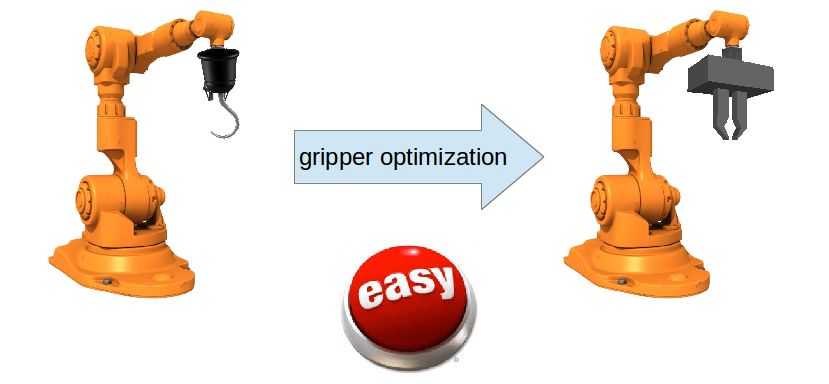
\includegraphics[width=0.6\textwidth]{images/motivation}
\end{center}
\end{frame}

\subsection{Zakres pracy}
\begin{frame}
\frametitle{Zakres pracy}
\begin{itemize}
\item \textbf{Opracowanie metryki opisującej jakość chwytaka}
\item \textbf{Parametryzacja szczęk chwytaka dwupalcowego}
\item \textbf{Zbadanie wpływu zmiany parametrów na jakość chwytaka -- symulacja}
\item \textbf{Zintegrowanie systemu oceny jakości w pętli optymalizacji}
\item \textbf{Optymalizacja chwytaków w kilku wybranych zadaniach}
\item Przeprowadzenie eksperymentów weryfikujących opracowaną metodę w praktyce
\item Stworzenie bazy danych i aplikacji do wspomagania projektowania
\item Wdrożenie opracowanej metody w praktyce
\end{itemize}
\end{frame}

\subsection{Automatyzacja}
\begin{frame}
\frametitle{Automatyzacja -- według XKCD}
\begin{center}
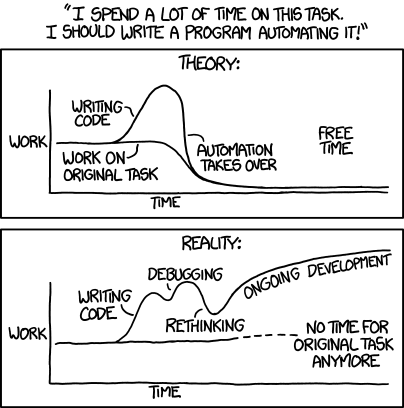
\includegraphics[width=0.4\textwidth]{images/automation}


Ukryty tekst: \textit{'Automating' comes from the roots 'auto-' meaning 'self-', and 'mating', meaning 'screwing'.}
\end{center}
\end{frame}

\subsection{Idea systemu}
\begin{frame}
\frametitle{Idea systemu}
\begin{center}
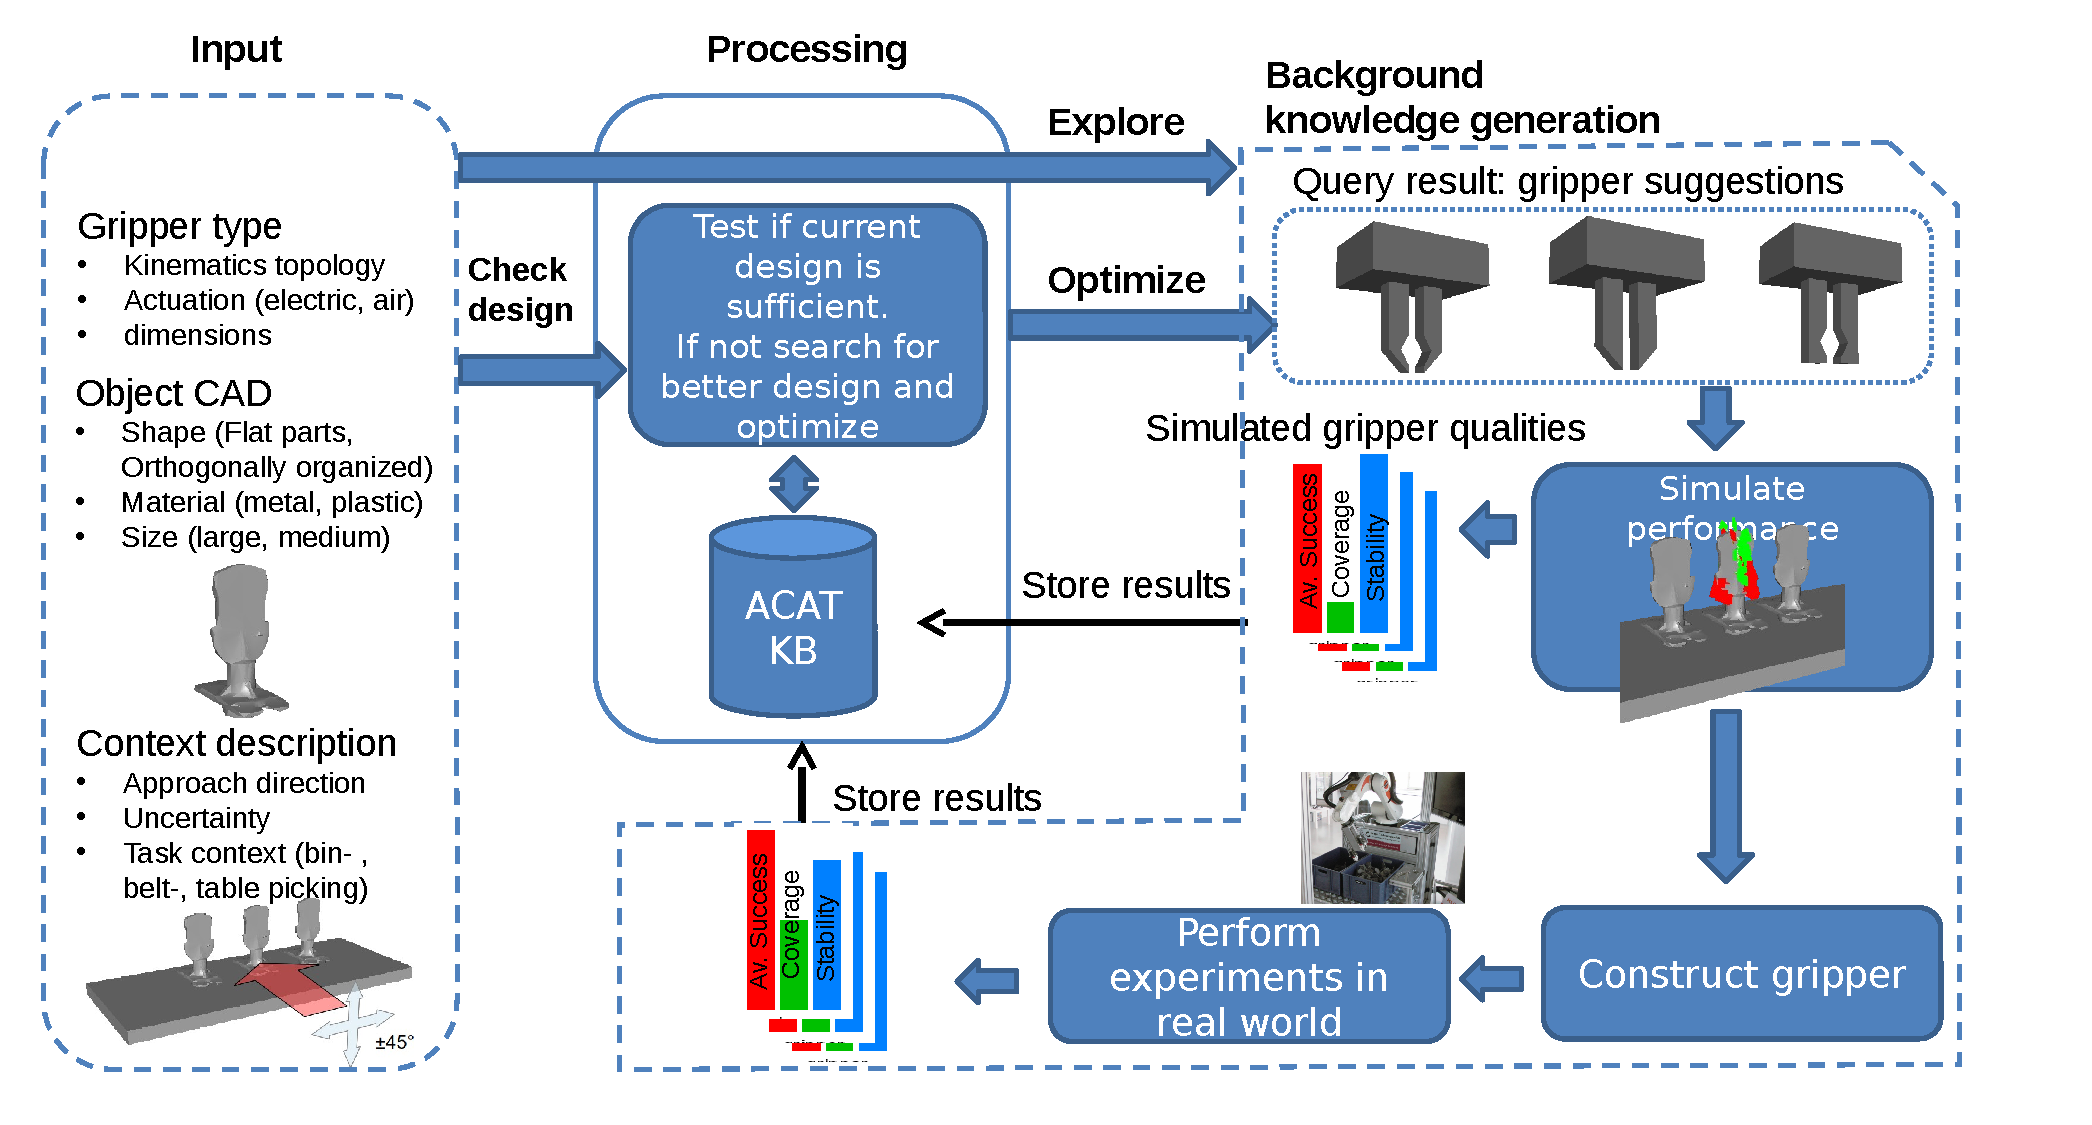
\includegraphics[width=1\textwidth]{images/bigpicture}
\end{center}
\end{frame}


\section{Metryka jakości chwytaka}
\subsection{METODA OCENY JAKOŚCI}
\begin{frame}
\frametitle{Metoda}
\begin{center}
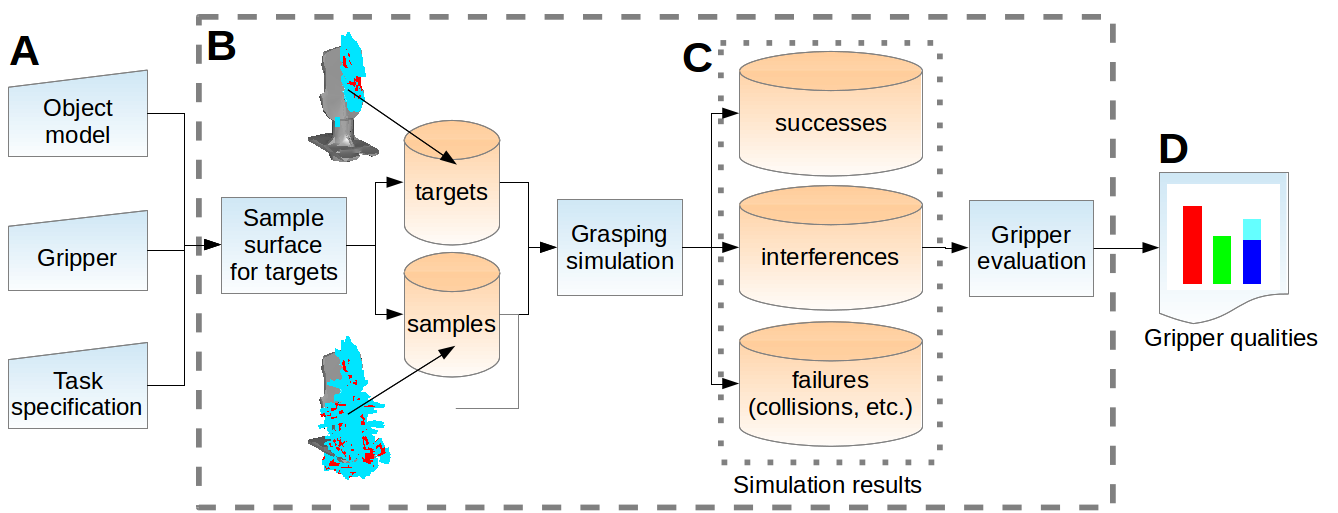
\includegraphics[width=0.9\textwidth]{images/process}
\end{center}
\end{frame}

\subsection{Symulacja}
\begin{frame}
\frametitle{Symulacja}
Sercem systemu jest dynamiczny symulator RobWorkSim.


Chwytanie może się zakończyć:
\begin{itemize}
\item sukcesem
\item chybieniem
\item kolizją
\item interferencją
\item \dots
\end{itemize}
\begin{block}{(Animacje)}
\movie[externalviewer]{\textit{Dobry} chwyt}{./movies/goodgrasp2.avi} \\
\movie[externalviewer]{\textit{Zły} chwyt}{./movies/badgrasp2.avi} \\
\movie[externalviewer]{\textit{Brzydki} chwyt}{./movies/badgrasp1.avi} \\
\end{block}
\end{frame}

\subsection{Success ratio}
\begin{frame}
\frametitle{\textit{Success ratio}}
\textbf{Success ratio} jest najbardziej intuicyjnym wskaźnikiem -- wskazuje jaki procent prób chwytania zakończył się sukcesem:

\begin{center}
$S = \frac{N_{successes}}{N_{filtered targets}}$

\vspace*{1cm}

\begin{tabular}{cc}
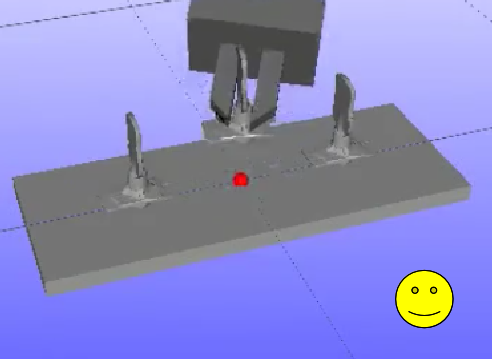
\includegraphics[width=0.3\textwidth]{images/goodgrasp1} &
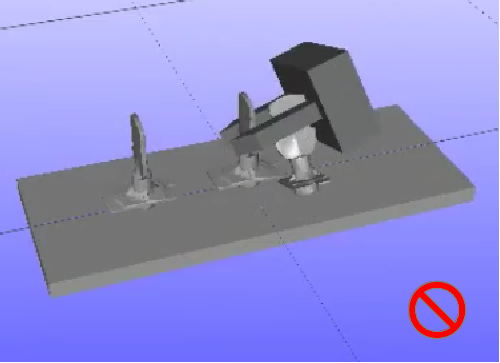
\includegraphics[width=0.3\textwidth]{images/badgrasp1}
\end{tabular}
\end{center}
\end{frame}

\begin{frame}
\frametitle{\textit{Coverage index}}
\textbf{Coverage index} wskazuje na objętość przestrzeni udanych chwytów pokrywającej chwytany obiekt przy użyciu danego typu chwytaka:


Wskaźnik ten oblicza się:
\begin{center}
$Q_{coverage} = \frac{N_{successes}+N_{interferences}}{N_{filtered\ samples}}$

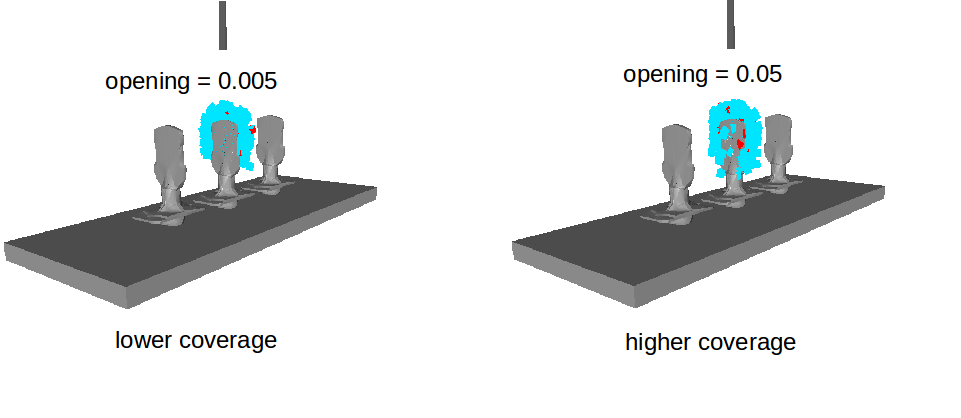
\includegraphics[width=0.66\textwidth]{images/coverage}
\end{center}
\end{frame}

\begin{frame}
\frametitle{\textit{Wrench indices}}
\textbf{Wrench indices} wskazują na średnią siłę (moment) zapewniany podczas chwytu -- dzięki mocnemu uchwytowi obiekt można poddać większemu przyspieszeniu, a zatem skrócić czas cyklu.

Obliczane są dwa wskaźniki:
\begin{itemize}
\item \textbf{Average wrench} -- średnia siła chwytu udanych prób
\item \textbf{Top wrench} -- średnia siła chwytu 20 \% najlepszych prób
\end{itemize}
\end{frame}

\begin{frame}
\frametitle{\textit{Stress index}}
\begin{tabular}{cc}
\begin{minipage}{0.5\textwidth}
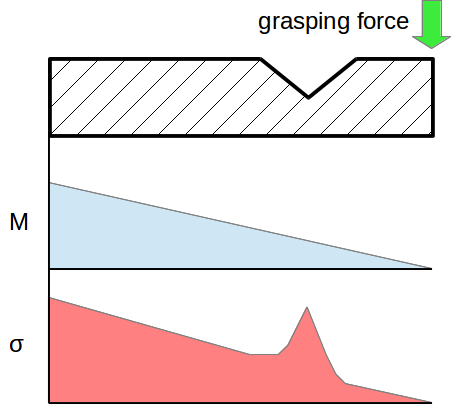
\includegraphics[width=1\textwidth]{images/stress}
\end{minipage}
 &
\begin{minipage}{0.5\textwidth}
\begin{itemize}
\item \textbf{Stress index} wskazuje na wytrzymałość danej geometrii palców
\item W optymalizacji wprowadza ograniczenie na minimalną grubość i maksymalną siłę chwytu
\item Im niższa wartość, tym lepiej!
\item Znajdujemy wartość $\sigma_{max}$
\end{itemize}
\end{minipage}

\end{tabular}
\end{frame}

\begin{frame}
\frametitle{\textit{Robustness index}}
\begin{itemize}
\item Nawet jeśli dana próba chwytu była udana, nie znaczy to, że po uwzględnieniu niepewności związanej z kalibracją i oceną pozycji, uda się powtórzyć dokładnie tę samą akcję
\item Każda próba jest sprawdzana ponownie pewną ilość razy, z uwzględnieniem zakłóceń w położeniu pozycji chwytaka i obiektu
\item \textbf{Robustness index} oblicza się: $Q_{robustness} = \frac{N_{perturbed\ successes}}{N_{successes}}$
\end{itemize}
\begin{center}
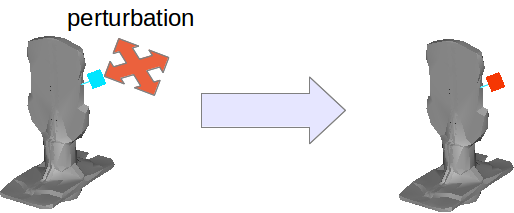
\includegraphics[width=0.5\textwidth]{images/robustness}
\end{center}
\end{frame}

\begin{frame}
\frametitle{\textit{Objective function}}
Ostatecznie, wskaźnik jakości chwytaka oblicza się jako średnią ważoną poszczególnych wskaźników, z uwzględnieniem funkcji kary związanej z ilością materiału zużytego na wykonanie szczęk:


\begin{align*}
Q = w_S \cdot S + w_C \cdot C + w_W \cdot W - w_\sigma \cdot \frac{\sigma_{max}}{\sigma_{limit}} - w_V \cdot V
\end{align*}
\end{frame}

\begin{frame}
\frametitle{Eksperymenty}
\centering
\begin{tabular}{|c|c|c|}
\hline
\emph{Rotor cap} & \emph{Dolt object} & \emph{Cylinder} \\ \hline
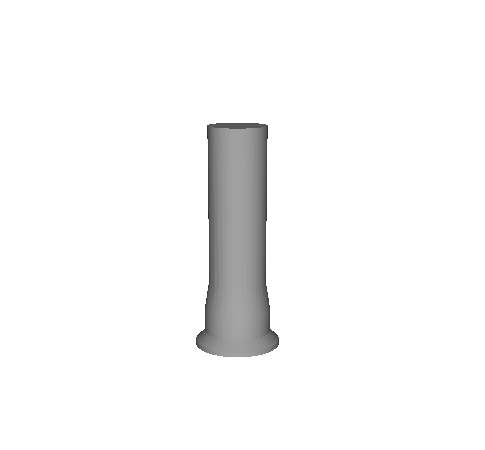
\includegraphics[width=0.3\textwidth]{images/rotorcap} &
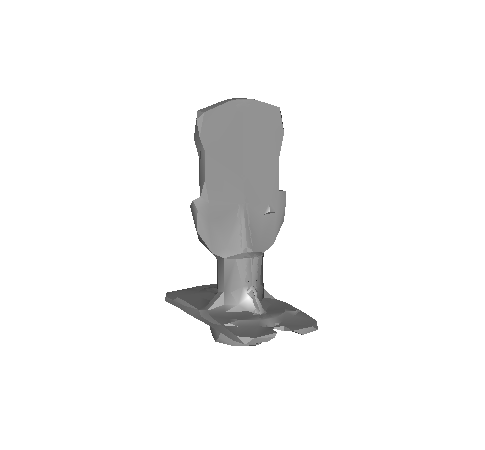
\includegraphics[width=0.3\textwidth]{images/dolt} &
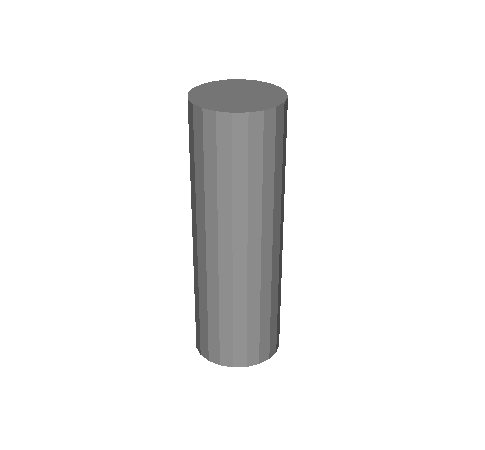
\includegraphics[width=0.3\textwidth]{images/cylinder} \\ \hline
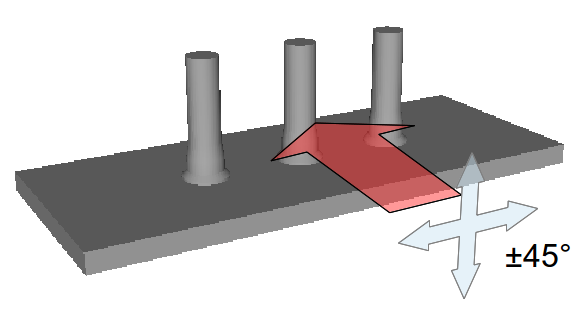
\includegraphics[width=0.3\textwidth]{images/rotor_task} &
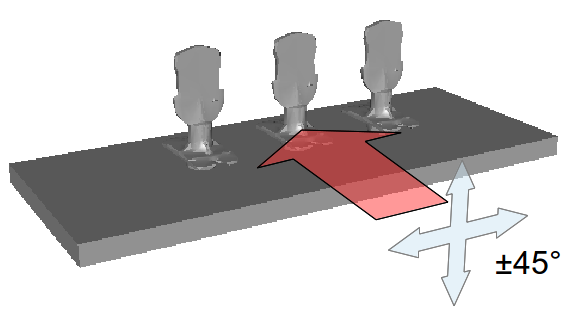
\includegraphics[width=0.3\textwidth]{images/dolt_task} &
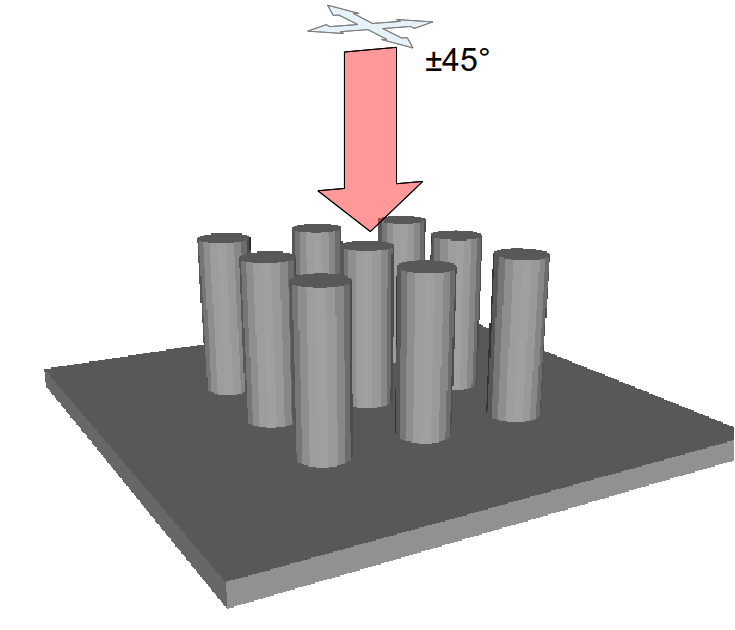
\includegraphics[width=0.3\textwidth]{images/cyl_task} \\ \hline
\end{tabular}
\end{frame}

\begin{frame}
\frametitle{Rezultaty}
\begin{center}
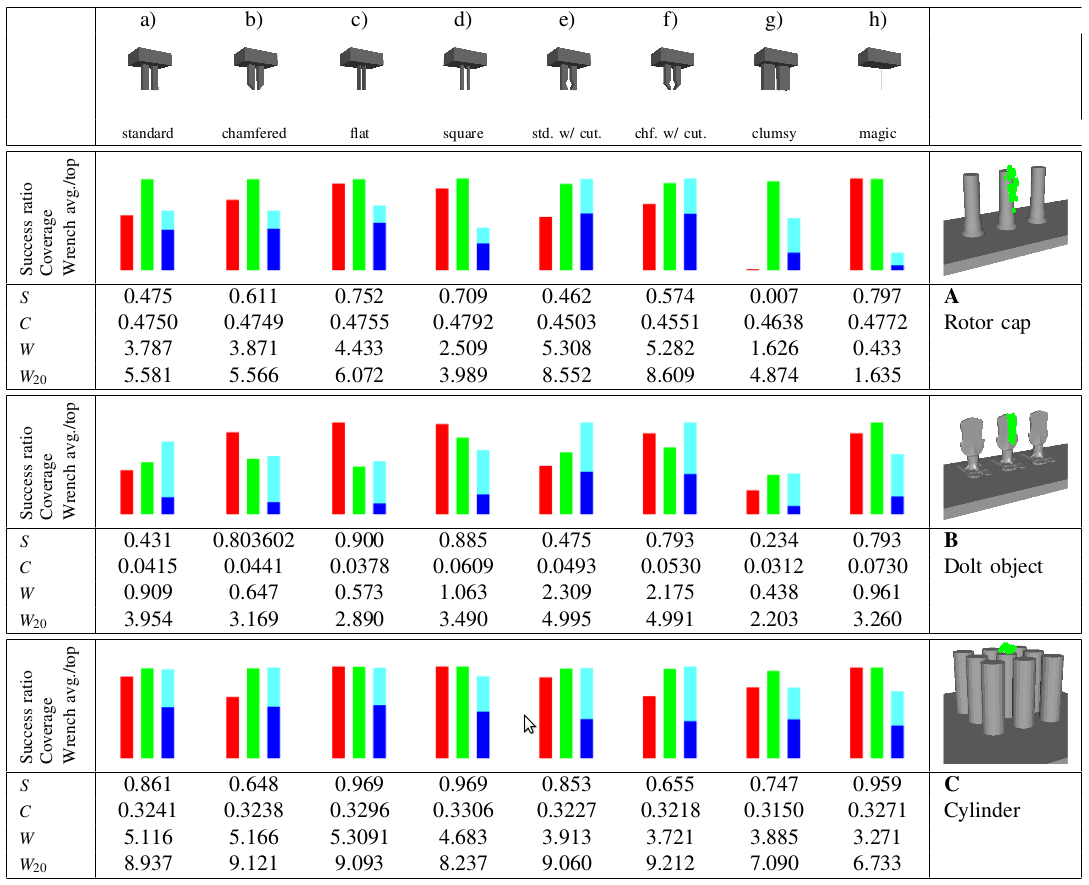
\includegraphics[width=0.9\textwidth]{images/oldresults}
\end{center}
\end{frame}


\section{Optymalizacja geometrii chwytaka}
\subsection{Wstęp}
\begin{frame}
\frametitle{OPTYMALIZACJA}
\begin{itemize}
\item W oparciu o opracowaną metodę oceny jakości, można wykorzystać różnorakie metody optymalizacji w celu ulepszenia istniejących, bądź wyznaczonych losowo projektów chwytaków
\item Konieczne jest wybranie odpowiedniej \textbf{parametryzacji},
\item Zweryfikowanie, czy \textbf{przebieg} funkcji jakości umożliwia optymalizację,
\item A następnie wybór odpowiedniej \textbf{metody} optymalizacji
\end{itemize}
\end{frame}

\subsection{Parametryzacja}
\begin{frame}
\frametitle{Parametryzacja geometrii szczęk}
\begin{tabular}{cc}
\begin{minipage}{0.5\textwidth}
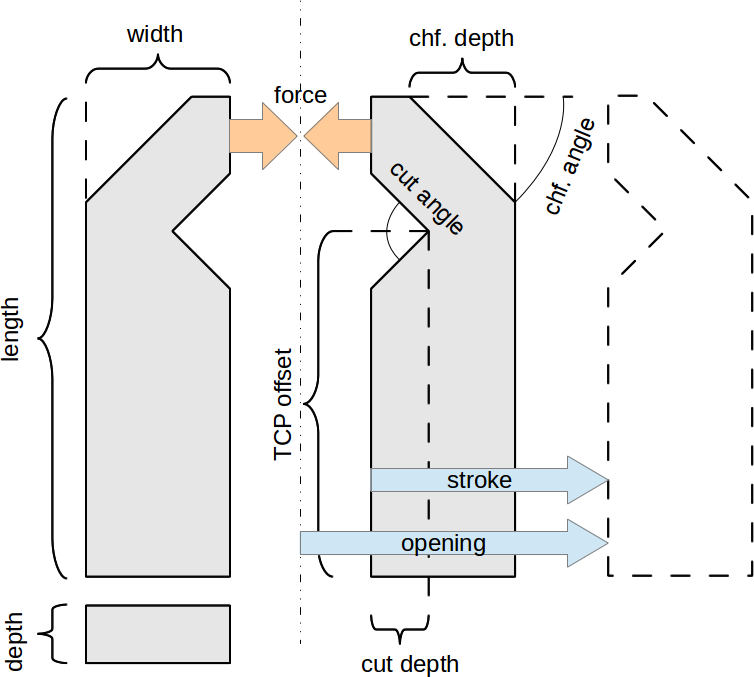
\includegraphics[width=1\textwidth]{images/parametrization}
\end{minipage} &
\begin{minipage}{0.5\textwidth}
\begin{tabular}{c|c|c}
\textbf{n.} & \textbf{parametr} & \textbf{zakres} \\ \hline \hline
1 & length & $0 \div 0.2$ \\ \hline
2 & width & $0 \div 0.05$ \\ \hline
3 & depth & $0 \div 0.05$ \\ \hline
4 & chf. depth & $0 \div width$ \\ \hline
5 & chf. angle & $0^\circ \div 90^\circ$ \\ \hline
6 & cut position & $0 \div length$ \\ \hline
7 & cut depth & $0 \div width$ \\ \hline
8 & cut angle & $0 \div 180^\circ$ \\ \hline
9 & tcp offset & $0 \div length$ \\ \hline
10 & stroke & $0 \div 0.1$ \\ \hline
11 & max. opening & $0 \div 0.1$ \\ \hline
12 & force & $0 N \div 100 N$
\end{tabular}
\end{minipage}
\end{tabular}
\end{frame}

\subsection{Krajobraz jakości}
\begin{frame}
\frametitle{\textit{Krajobraz} jakości}
Poprzez wybór pewnego punktu początkowego w przestrzeni parametryzacji, a następnie modyfikację poszczególnych parametrów, możemy wyznaczyć wycinki przestrzeni jakości:

\begin{center}
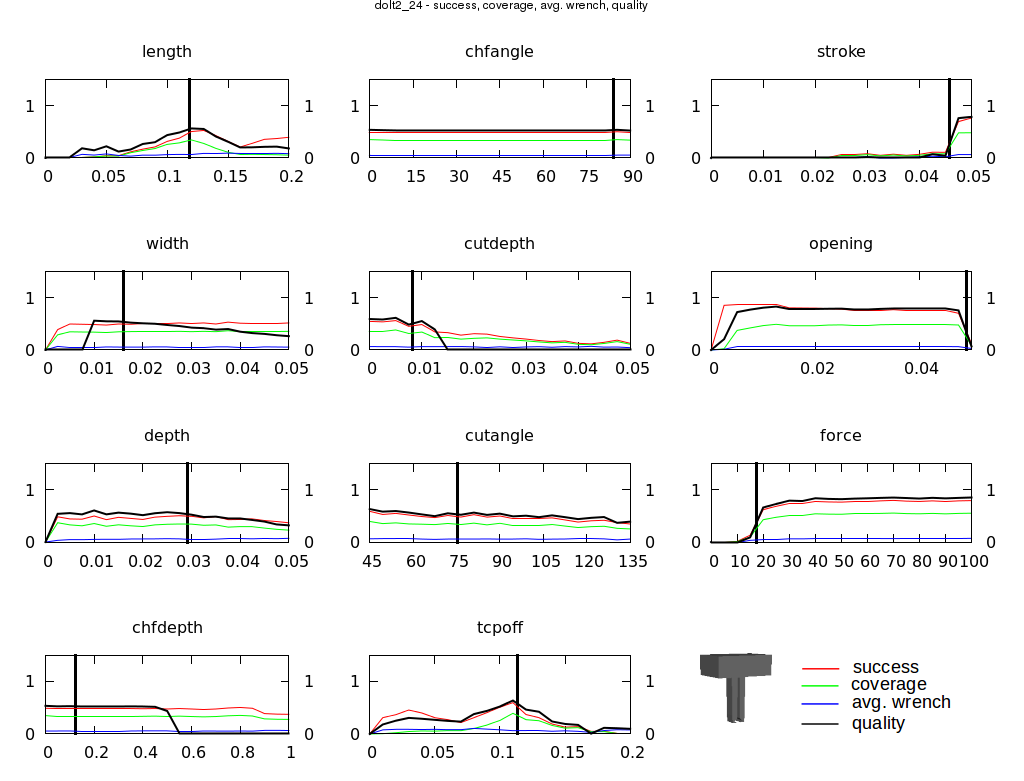
\includegraphics[width=0.8\textwidth]{images/dolt2_24_3}
\end{center}
\end{frame}

\subsection{Metoda optymalizacji}
\begin{frame}
\frametitle{Metoda optymalizacji}
\begin{tabular}{cc}
\begin{minipage}{0.5\textwidth}
Jako metodę optymalizacji wybrano \textbf{metodę gradientową}.
\vspace{2cm}
\begin{block}{\textit{Gradient descent}}
\movie[externalviewer]{\textit{Animacja}}{images/ani1.gif}
\end{block}
\end{minipage}
 &
\begin{minipage}{0.5\textwidth}
Algorytm:
\begin{itemize}
\item Wygeneruj punkty w przestrzeni parametryzacji w bezpośrednim otoczeniu punktu początkowego w danym kroku
\item Wyznacz przebieg funkcji jakości w poszczególnych wymiarach przestrzeni
\item Wyznacz gradient
\item Wykonaj krok w oparciu o wyznaczony gradient
\end{itemize}
\end{minipage}
\end{tabular}
\end{frame}

\subsection{Rezultaty}
\begin{frame}
\frametitle{Optymalizacja losowa}
Dla wybranych zadań wygenerowano heurystycznie zbiór przypadkowych parametryzacji chwytaków, a następnie dokonano optymalizacji niektórych z nich.

\begin{center}
\begin{tabular}{|c|c|c|}
\hline
\textbf{1. all directions} & \textbf{2. from top} & \textbf{3. from side} \\
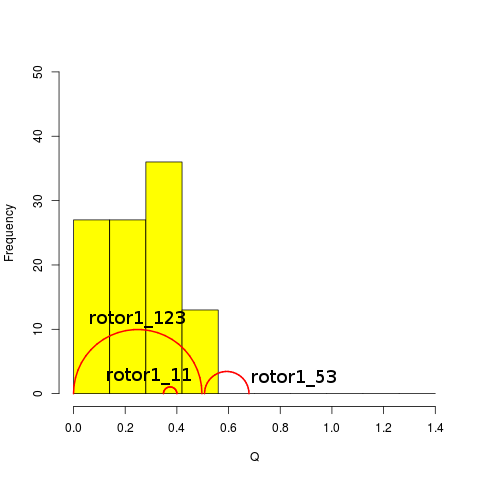
\includegraphics[width=0.3\linewidth]{images/s100_rotor1_opt} &
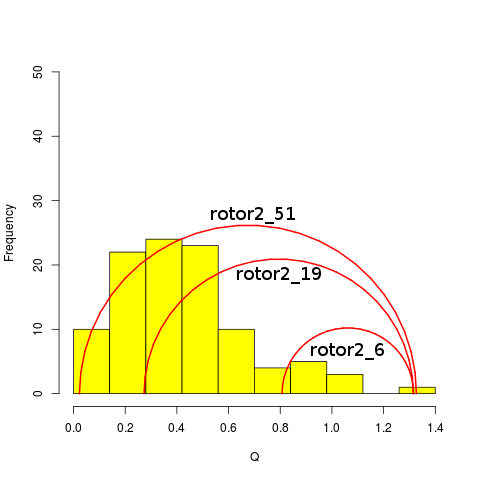
\includegraphics[width=0.3\linewidth]{images/s100_rotor2_opt} &
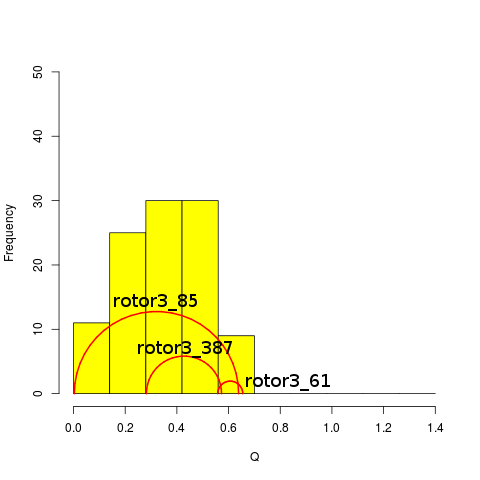
\includegraphics[width=0.3\linewidth]{images/s100_rotor3_opt} \\ \hline
\end{tabular}
\end{center}
\end{frame}

\subsection{Przykład optymalizacji}
\begin{frame}
\frametitle{Przykład optymalizacji}
\begin{tabular}{cc}
\begin{minipage}{0.5\textwidth}
Jak wygląda ewolucja przykładowego projektu?
\vspace{1cm}
\begin{block}{Ewolucja}
\movie[externalviewer]{\textit{Animacja}}{images/s100_rotor3_387.gif}
\end{block}
\end{minipage}
 &
\begin{minipage}{0.5\textwidth}
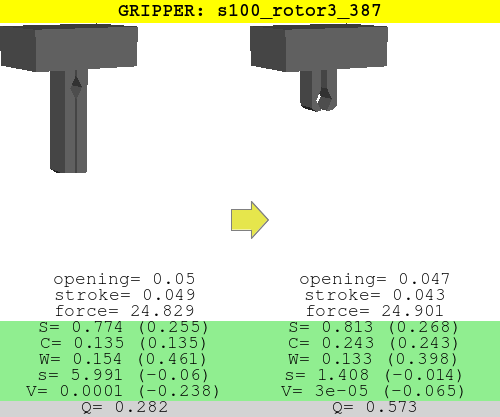
\includegraphics[width=\linewidth]{images/s100_rotor3_387_result}
\end{minipage}
\end{tabular}
\end{frame}

\section{Koniec}
\subsection{Dalsze prace}
\begin{frame}
\frametitle{Plany na przyszłość}
\begin{itemize}
\item Wprowadzenie dodatkowych kryteriów jakości (np. \textit{alignment}, ...
\item Rozszerzenie możliwości parametryzacji na inne kształty i typy chwytaków
\item Stworzenie bazy danych z projektami i rezultatami oceny
\item Opracowanie heurystycznej metody szybkiej oceny i optymalizacji na podstawie zgromadzonych danych
\item Eksperymenty weryfikujące metodę w praktyce
\item Opracowanie aplikacji wspomagającej projektowanie chwytaków
\item Wdrożenie opracowanej metody w wybranym zadaniu przemysłowym
\end{itemize}
\end{frame}

\subsection{Podsumowanie}
\begin{frame}
\frametitle{Podsumowanie}
\begin{itemize}
\item Opracowano metodę oceny jakości chwytaka na podstawie symulacji
\item Wybrano parametryzację geometrii szczęk chwytaka dwupalcowego
\item Zastosowano metodę optymalizacji w oparciu o opracowaną funkcję jakości w wybranej przestrzeni parametryzacji
\end{itemize}


Publikacje:
\begin{itemize}
\item Adam Wolniakowski, Konstantsin Miatliuk, Norbert Kruger, Jimmy A. Rytz ``\textit{Automatic evaluation of task-focused parallel jaw gripper design}''
\item Adam Wolniakowski, Jimmy A. Jorgensen, Konstantsin Miatliuk, Henrik Gordon Petersen, Norbert Kruger ``\textit{Task and context sensitive optimization of gripper design using dynamic grasp simulation}''
\end{itemize}
\end{frame}

\subsection{Koniec}
\begin{frame}
\frametitle{Koniec}
Dziękuję za uwagę!
\end{frame}

\end{document}